%
% developers.tex
%
% (c)2013 UAF. Author: Anton V. Kulchitsky
%
% Developers' documentation to Siku, COUPi Sea Ice DEM model
%

\documentclass[pdftex,12pt]{report}

\usepackage{graphicx}
\usepackage[usenames]{color}
\usepackage{longtable}
\usepackage{bm}
\usepackage{amsmath}
\usepackage{amsthm}
\usepackage{amssymb}


\usepackage{tocbibind}   % for including bibliography into TOC
                         % options: notbib, notindex, nottoc,
                         %          notlof, notlot

\usepackage{ifthen}
%\usepackage{calc}
%\usepackage{ctable}      % for footnotes in tables

\usepackage[colorlinks,linkcolor=blue]{hyperref}

\usepackage[margin=1in]{geometry}

%temp color bundle ----
\usepackage[usenames,dvipsnames]{xcolor}
\pagecolor{PineGreen}
%\pagecolor{Aquamarine}
%----------------------

%==========================

\newcommand{\HRule}{\rule{\linewidth}{0.5mm}}

\newcommand{\forloop}[5][1]%
{%
  \setcounter{#2}{#3}%
  \ifthenelse{#4}%
             {%
               #5%
               \addtocounter{#2}{#1}%
               \forloop[#1]{#2}{\value{#2}}{#4}{#5}%@
             }%
             % Else
             {%
             }%
}%

\newcommand{\coupi}{\textsc{cou}{\LARGE $\pi$}}
\newcommand{\coupiice}{\textsc{cou}{\LARGE $\pi$}\textsc{-ice}}

\theoremstyle{definition}
\newtheorem{defn}{Definition}

\theoremstyle{plain}
\newtheorem{thm}{Theorem}

%{{ //THE ARE SOME ADDITIONAL COMMANDS DEFINED BY ANTON KULCHITSKY
\newcommand{\odt}[1]{\mathop{ \frac{d #1}{dt} }}
\newcommand{\oddt}[1]{\mathop{ \frac{d^2 #1}{dt^2} }}
\newcommand{\dii}[2]{\mathop{ \frac{\partial #1}{\partial #2} }}
\newcommand{\ddii}[2]{\mathop{ \frac{\partial^2 #1}{\partial #2^2} }}
\newcommand{\diit}[1]{\mathop{ \frac{\partial #1}{\partial t} }}
\newcommand{\diir}[1]{\mathop{ \frac{\partial #1}{\partial r} }}
\newcommand{\diix}[1]{\mathop{ \frac{\partial #1}{\partial x} }}
\newcommand{\diiy}[1]{\mathop{ \frac{\partial #1}{\partial y} }}
\newcommand{\diiz}[1]{\mathop{ \frac{\partial #1}{\partial z} }}
\newcommand{\diip}[1]{\mathop{ \frac{\partial #1}{\partial p} n}}
\newcommand{\diis}[1]{\mathop{ \frac{\partial #1}{\partial s} }}
\newcommand{\diith}[1]{\mathop{ \frac{\partial #1}{\partial \theta} }}
\newcommand{\diiph}[1]{\mathop{ \frac{\partial #1}{\partial \varphi} }}
\newcommand{\erf}{\mathop{\mathrm{erf}}}
\newcommand{\rot}[1]{\mathop{\nabla\times#1}}
\newcommand{\Ec}{{\cal E}}

% Update the following commands if you would like to change the
% default notation for vectors, points, matrices/operators, and
% quaternions.
\newcommand{\vct}[1]{{\vec{#1}}} 
\newcommand{\mtr}[1]{{\bm{#1}}}
\newcommand{\untqtrn}[1]{{\hat{\bm{#1}}}}
\newcommand{\untvct}[1]{{\hat{#1}}}
\newcommand{\pnt}[1]{{\vct{#1}}}

\renewcommand{\Re}[1]{\mathop{\text{Re}\,#1}}
\renewcommand{\Im}[1]{\mathop{\text{Im}\,#1}}


% coupi date command generated by ./bootstrap.py
\include{date}
\newcommand{\acknowledgements}{

  {\large This study is sponsored by the University of Alaska Coastal
    Marine Institute. Study collaboration and funding were provided by
    the U.S. Department of the Interior, Bureau of Ocean Energy
    Management, Environmental Studies Program under Agreement Number
    M13AC00001.}

  \medskip{\large The matching funds are provided by Institute of
    Northern Engineering, University of Alaska Fairbanks and by Oregon
    State University.}

  \medskip{\large This work was supported in part by a grant of HPC
    resources from the Arctic Region Supercomputing Center at the
    University of Alaska Fairbanks.}

 \medskip}


\newcommand{\mytitleone}{Siku}
\newcommand{\mytitletwo}{\Large Sea Ice Discrete Element Method Model}
\newcommand{\myexttitle}{\Large Final Report and Documentation}

\begin{document}
%
% titlepage.tex

% Template to create title page for all documentation in the
% project. It contains all authors, contributors, and consultants
% names. Change it if you add more contributors or consultants. You
% also want to change it to change the look and feel of the title
% pages everywhere through final documentation
%


\begin{titlepage}
\begin{center}
% Upper part of the page

\includegraphics[width=0.2\textwidth]{../pics/logoice.pdf}\\[4.5cm]

%\textsc{\LARGE University of Alaska Fairbanks}\\[1.5cm]
% \textsc{\Large Final year project}\\[0.5cm]

% Title
\HRule \\[0.4cm]

{\huge\bfseries \mytitleone}\\[0.4cm]
\ifthenelse{\equal{\mytitletwo}{0}}{}%
                  {{\huge\bfseries  \mytitletwo}\\[0.4cm]}
\ifthenelse{\equal{\myexttitle}{0}}{}%
                  {{\large\bfseries  \myexttitle}\\[0.4cm]}

\HRule \\[1.5cm]

% Author and supervisor
\begin{minipage}{0.4\textwidth}
\begin{flushleft} \large
\emph{Authors:}\\
Anton V \textsc{Kulchitsky}\\
Jennifer \textsc{Hutchings}\\
Jerome B \textsc{Johnson}
\end{flushleft}
\begin{flushleft} \large
%{\emph{Contributors:} } \\
%Paul \textsc{Duvoy}\\
%Ben \textsc{Nye}
\end{flushleft}
\end{minipage}
\begin{minipage}{0.4\textwidth}
\vspace{42pt}
\begin{flushright} \large
%\emph{Consultants:}\\
%Mark \textsc{Hopkins}\\
%Otis \textsc{Walton}
\end{flushright}
\end{minipage}

\vfill

% Bottom of the page
{\large \coupidate}

\end{center}
{\hfill\textit{branch:} \branchname}

{\hfill\textit{version:} \coupiversion}

\end{titlepage}


\pagestyle{headings}
\vspace*{\fill}
\acknowledgements
\pagebreak
\tableofcontents
\pagebreak

%=====================================================================
% FILE: introduction.tex

\chapter{Introduction}

%---------------------------------------------------------------------
\section{Basic Information}

Siku is written on a subset of C++ language. Please, see
Sec.~\ref{sec:programing-policy} for strict programming policy.

%---------------------------------------------------------------------
\section{Software Requirements}

To compile and use the model, the following packages are required:
\begin{enumerate}
\item Python 3.0 or higher
  \begin{enumerate}
  \item \texttt{mathutils} from blender project. 
    See \url{https://code.google.com/p/blender-mathutils/}.
  \item \texttt{netcdf4-python} (recommended if you need import
    NetCDF4 forcing files).
  \item \texttt{numpy}
  \item \texttt{shapefile} (known also as \texttt{pyshp}).
  \end{enumerate}
\item HDF5 version 1.8 or higher.
\item NetCDF4 version 4.1.1 or higher.
\item GSL version 1.16 or higher.
\item Boost library version 1.53 or higher.
\item OpenGL Mathematics (GLM) version 0.9.6.1 or higher.
\item \LaTeX\/ for creating documentation.
\end{enumerate}

The packages that are necessary to compile the core are checked during
the configuration step. Python libraries are not checked.

%---------------------------------------------------------------------
\section{Programming Policy}\label{sec:programing-policy}

A strict programming policy is enforced to keep the code clean and
rational. This policy is strictly enforced in particular due to usage
of such an obscure, overloaded and heavy language as C++.

%----------------------------------------------------------------------
\section{Development Policy}



%=====================================================================
%FILE: coordinates.tex

\chapter{Ice Element Location and Position}

\section{Introduction}

Let an ice element be considered as a flat (2D) rigid body in a form
of convex polygon moving on a spherical surface. The goals of this
chapter are
\begin{itemize}
  \item Find a suitable description of position and orientation of the
    ice element;
  \item Derive position integraion equations;
  \item Build an integration numerical algorithm to update position
    and orientation of the ice element;
  \item Describe coordinate transformations used in the model.
\end{itemize}

\section{Equivalence to 3D Rigid Body Rotations}

\begin{figure}
  \center
  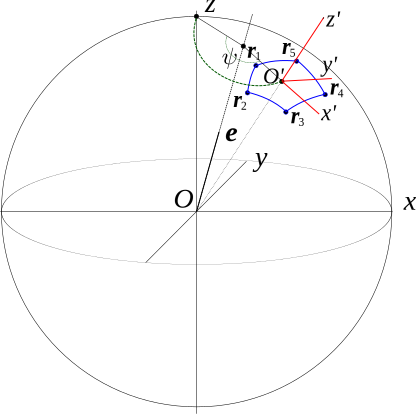
\includegraphics[width=0.5\textwidth]{pics/sphere-dynamics.pdf}
  \caption{Coordinates}
  \label{fig:coordinates}
\end{figure}

It is easy to see (but not so easy to find out) that the motion of an
ice element on the surface of a sphere is equivalent to a rotation of
a rigid body around the center of the sphere. Such a rigid body can be
considered to be a pendulum with a massive weight to be a material
polygon which center of mass is connected to the center of the sphere
by a massless rod. The center of the sphere does not move and is a
center of the rotation. This set up is shown in
Figure.~\ref{fig:coordinates}.

It also can be visualized as a rotation of the rigid sphere shell
around its center with all the mass concentrated inside a single
polygon patch -- an ice element.

The representation of an ice element as a 3D constrained rotating
rigid body provides a useful instrument to describe exact position and
orientation of an ice element. The rigid body rotation around a point
can be described by unit quaternions a.k.a
versors~\cite{bib:graf2008quaternions, bib:waldvogel2008quaternions,
  bib:arribas2006quaternions, bib:nemes2013perturbed}. The main
advantage of using quaternions instead of, say, spherical coordinates
with a rotation angle is that every point on a sphere is treated
exactly the same way as any other point. The density of coordinate
lines do not change from point to point and no critical points are
present. The quaternion representation also allows to perfom many
coordinate transformations without involving trigonometry, store
orientation information very compactly, and the formulas of all
necessary operations are simple and short. \textbf{A single quaternion
  is sufficient to uniqly describe the position and orientation of an
  ice element}.

%----------------------------------------------------------------------
\section{Coordinate Systems and Frames}\label{sec:frames}

When describing different values such as positions or vectors we use 2
different types of reference points or ``frames'' depending on
convenience:
\begin{itemize}
\item Global Frame, connected to the Earth and rotating with the
  Earth;
\item Local Frames, a reference point connected to a particular ice
  element.
\end{itemize}

For describing elements in Global Frame, we use 3 different coordinate
system:
\begin{itemize}
\item Geographical coordinates (latitude $\varphi$ and longitude
  $\lambda$). They used only for import or export elements and never
  used internally. We provide trasformation from and to geographical
  coordinates.
\item Spherical coordinates ($\phi=\lambda$, $\theta=\pi/2-\varphi$).
\item 3D extrinsic Cartesian coordinates $(x',y',z')$.  Its center
  coincides with the center of the Earth $O$, $z'$ is directed along
  Earth's axis of rotation towards the North, $x'$ direction is a
  direction to 0 meridian, and $y'$ direction is chosen perpendicular
  to $x'$ and $z'$ to form a right coordinate system. These
  coordinates satisfy the constrain ${x'}^2+{y'}^2+{z'}^2=R^2$.
\item 3D normalized (dimensionless) extrinsic Cartesian coordinates
  $(x,y,z)$. Same as above but all projected to a unit sphere such
  that ${x}^2+{y}^2+{z}^2=1$.  \textit{These are the main global coordinates
  internally used in the Core for all the computations.}
\end{itemize}

We use Global Frame only when considering interaction between two ice
elements. In all other cases we transform global coordinates into a
local frame first and then produce the computations.

The transformation between extrinsic coordinates and
geographic/spherical coordinates are performed using the following
formulas:
\begin{equation}\label{eq:extrinsic}
  \left\{
  \begin{aligned}
    \theta &= \pi/2 - \varphi,\\
    \phi &=\lambda.\\
  \end{aligned}
  \right.\qquad\left\{
  \begin{aligned}
    x &= \sin\theta\cos\phi, \\
    y &= \sin\theta\sin\phi, \\
    z &= \cos\theta.\\
  \end{aligned}
  \right.
\end{equation}

Local coordinates $(X,Y,Z)$ are the coordinates that have its center
in the center of mass of the ice element. The axis are directed such
that they would coincide with global frame normalized extrinsic
coordinates $(x,y,z)$ after application of the rotation described by
the quaternion $\untqtrn{q}$ linked to the ice element.

Global extrinsic coordinates for any point $\pnt{p}$ are restored from
local coordinates $\pnt{P}$ by applying the rotation matrix recovered
from quaternion:
\begin{equation}
  \pnt{p} = \mtr{R}(\untqtrn{q})\cdot\pnt{P}
\end{equation}
Rotation matrix can be recovered from quaternion as described in
Section~\ref{sec:rotquat}.

%----------------------------------------------------------------------
\section{Initial Frame Relation}

To relate two different frames, we have to introduce initial
quaternion $\untqtrn{q}_0$. Later we will provide a first order
differential equation for the evolution of the quaternion. However, we
have to find this initial quaternion to be able to resolve the
evolution.

We found a simple way to set this initial position
quaternion. Initially, we have initial coordinates of the polygon
representing the ice elements in some of Global Frame coordinates. To
find initial quaternion we will do the following
\begin{enumerate}
\item Find center of mass of the polygon in global frame.
\item Find a quaternion such that when applied, it moves the center of
  mass into the North Pole. There are an infinite number of such
  rotation quaternions, so we pick one.
\item We introduce initial local coordinates based on this initial
  quaternion such that they will coincide with extrinsic coordinates
  after the transformation. All vertices coordinates $\pnt{P}_i =
  (X_i,Y_i,Z_i)$ are computed then. They will never change with time.
\end{enumerate}

There is an uncertainty in quaternion choice that initially would
transpose the center of ice element into North pole. Let us choose the
quaternion that transpose the center of the ice element as follows.

Suppose we have coordinates of the center of mass in Global Frame in
Extrinsic coordinates: $\pnt{c}=(c_x,c_y,c_z)$, then we restore the
transformation as a rotation along big circle to match $\pnt{c}$ with
North Pole as follows:
\begin{equation}
  \untqtrn{q_0} = \cos{\theta/2} + \untvct{e}\sin{\theta/2},\qquad \untvct{e} =
  \vct{c}\times\untvct{e_z}/|\vct{c}\times\untvct{e_z}|, \quad \theta =
  \arccos{c_z/|\vct{c}|}.
\end{equation}
$\theta$ is spherical coordinates of $\pnt{c}$. The rotation axis is
perpendicular to $\pnt{c}$ and direction to the North. Reminder: we
use a convention that vectors and scalars are all a subset of
quaternions and can be added to each other to make a new quaternion.

%% -------------------------------------------------------------------

\section{Position Update Equation}

Suppose we know the vector of angular velocity of our ``pendulum''
$\vec{\omega}$. Please, notice that this is 3D angular velocity
vector, not a rotation rate of the ice element. Later we will see how
to calculate it from the velocity and rotation rate of the ice element
itself. In this case we have the following expression for updating
orientation quaternion
\begin{equation}
  \dot{\untqtrn{q}} = \frac{1}{2}\vct{\omega}\circ\untqtrn{q}.
\end{equation}
Where $\dot q=dq/dt$.  Let $\vct{\Omega}$ be the same angular velocity
vector expressed in Local frame
coordinates. Using~\eqref{eq:transform} we can derive the main
position equation:
\begin{equation}\label{eq:positionomega}
  \dot{\untqtrn{q}} = \frac{1}{2}\untqtrn{q}\circ\vct{\Omega},
\end{equation}
While developing \coupi\/ we created a very neat scheme to solve this
type of equations. This scheme will be described here later based on
\coupi\/ documentation.

%% -------------------------------------------------------------------

\section{Placement Numerical Integration}

Let us describe the numerical solution of the
equation~\eqref{eq:positionomega}.  

Let $\vct{\Omega}^{n+1/2} = \vct{\Omega}(t+\Delta t/2)$ (and this
value we will actually find on the dynamic stage),
$\untqtrn{q}^{n}=\untqtrn{q}(t)$,
$\untqtrn{q}^{n+1}=\untqtrn{q}(t+\Delta t)$. The 2nd order scheme for
the equation above will be
\begin{equation}
  \untqtrn{q}^{n+1} = \untqtrn{q}^n + \frac{\Delta t}{4} 
  (\untqtrn{q}^{n}+\untqtrn{q}^{n+1})\circ
  \vct{\Omega}^{n+1/2}.
\end{equation}
Collecting all next step values on the left side and taking into
account that quaternion product is not commutative, we have
\begin{equation}\label{eq:scheme}
  \untqtrn{q}^{n+1}\circ\left( 1 - \frac{\Delta t}{4}\vct{\Omega}\right) = 
  \untqtrn{q}^{n}\circ\left( 1 + \frac{\Delta t}{4}\vct{\Omega}\right).
\end{equation}
We removed index $n+1/2$ from $\vct{\Omega}$ to make it easier to
read. Brackets in~\eqref{eq:scheme} are conjugate
quaternions. Using relation $\untqtrn{q}\circ\untqtrn{\bar{q}} = |q|^2$ we have
\begin{equation}
  \untqtrn{q}^{n+1}\circ\left( 1 - \frac{\Delta
    t}{4}\vct{\Omega}\right)\circ\left( 1 + \frac{\Delta
    t}{4}\vct{\Omega}\right) = \untqtrn{q}^{n}\circ\left( 1 + \frac{\Delta
    t}{4}\vct{\Omega}\right)^2.
\end{equation}
\begin{equation}
  \untqtrn{q}^{n+1}\left( 1 +\frac{ \Omega^2\,\Delta
    t^2}{16}\right) = \untqtrn{q}^{n}\circ\left( 1 + \frac{\Delta
    t}{4}\vct{\Omega}\right)^2.
\end{equation}
\begin{equation}
  \untqtrn{q}^{n+1} = \untqtrn{q}^{n}\circ\left( 1 + \frac{\Delta
    t}{4}\vct{\Omega}\right)^2 / \left( 1 +\frac{ \Omega^2\,\Delta
    t^2}{16}\right)
\end{equation}
For any vector $\vct{a}$ using product Eq.~\eqref{eq:quatproduct} we
have
\begin{equation}
  (1+\vct{a})^2 = (1+\vct{a})\circ(1+\vct{a}) =
  1 - a^2 + 2\vct{a}.
\end{equation}
Then, we have
\begin{equation}
  \untqtrn{q}^{n+1} = \untqtrn{q}^{n} \circ \left(1 - \frac{\Omega^2\,\Delta t^2}{16} +
  \frac{\Delta t}{2}\,\vct{\Omega} \right) / \left( 1 +\frac{ \Omega^2\,\Delta
    t^2}{16}\right)
\end{equation}
Let us introduce the following quaternion
\begin{equation}
  \untqtrn{p} = \left(1 - \frac{\Omega^2\,\Delta t^2}{16} + \frac{\Delta
    t}{2}\,\vct{\Omega} \right) / \left( 1 +\frac{ \Omega^2\,\Delta
    t^2}{16}\right),
\end{equation}
then integration formula will have the form
\begin{equation}
  \untqtrn{q}^{n+1} = \untqtrn{q}^{n} \circ \untqtrn{p}.
\end{equation}
Computation wise it is a significant improvement over
\cite{bib:Walton-Braun-1993} quaternion integration formula or
trigonometric approach like in \cite{bib:gpugems3-harada-2008}.

It is easy to see that $|\untqtrn{p}|=1$ and hence this formula does not
change the absolute value of unit quaternion. However, round-off
errors might accumulate in time shifting the absolute value of
$\untqtrn{q}$ from 1. To ensure we are working within unit quaternion
algebra, a renormalization should be done occasionally
\begin{equation}
  \untqtrn{q} \leftarrow \untqtrn{q}/|q|.
\end{equation}


%=====================================================================
%%% File: dynamics.tex

\chapter{Dynamics}

%----------------------------------------------------------------------

\section{Introduction}

The main problem in dynamics is to calculate 3D ``pendulum'' angular
velocity $\vct{\Omega}$ in ice-element reference frame. This vector
can be calculated exactly using 3D dynamics of a rigid body with
constraints. However, it is not necessary. A much simpler way should
be sufficient if we suppose that the ice-element size is much smaller
than the radius of the Earth. This is equivalent to the assumption
that the ice element is flat.

In spite of this assumptions we are not solving 2D cartesian
problem. All we are saying is that we are considering the dynamics on
a sphere with locally flat ice elements.

%----------------------------------------------------------------------

\section{Dynamics in ice-element reference frame}

As ice-element reference frame is a standard cartesian coordinates and
we assume that the ice-element is a flat 2D ridig body, its velocity
and rotation rate can be calculated simply by the following equations
\begin{equation}\label{eq:dynamicsset}
  \dot{V_x} = F_x/m, \qquad \dot{V_y} = F_y/m, 
  \qquad \dot\Omega_z = N/I,
\end{equation}
where $(F_x,F_y)$ are external forces that include all driving forces,
integral forces from interaction with other ice-elements, and Earth
Coriolis force, $m$ is the total mass of the ice element, $I$ is a
moment of inertia around $Z$ axis, and $N$ is a total torque
calculated in the center of mass $\vct{C}$ that includes a torque from
interaction with other ice elements and possible torque that can be
calculated from the integral $(\nabla\times F)_z$ of the driving
forces over the ice element (TODO: discuss with Jenny).

%----------------------------------------------------------------------

\section{Restoring 3D angular velocity}

It is pretty clear that if we know $V_x$, $V_y$, and $\Omega_z$, we
can restore $\vct{\Omega}$ as follows: 
\begin{equation}
  \vct{\Omega}= (-V_y/R, V_x/R, \Omega_z)^T.
\end{equation}
Indeed, $V_x$ is directed normal to $Z$ and tends to rotate the
``pendulum'' around $Y$ axis with $V_x/R$ rate. The rotation
direction is ``right'' and that is exactly $\Omega_y$. Same
considerations show that $|\Omega_x| = V_y/R$ and we need to choose
``-'' as a sign to take into account the right direction.

Taking this into account, we can rewrite the dynamics ecuations for
global angular velocity vector in Local frame:
\begin{equation}\label{eq:dynamicsH}
  \dot{\vct{\Omega}} = \vct{H} = \left( -\frac{F_y}{mR}, \frac{F_x}{mR},
  \frac{N}{I} \right)^T.
\end{equation}

%----------------------------------------------------------------------

\section{Dynamics Integration}

A straightforward 2nd order in time scheme is applicable for
Eq.~\eqref{eq:dynamicsH}:
\begin{equation}
  \left\{
  \begin{aligned}
  \Omega_x^{n+1/2} &= \Omega_x^{n-1/2} - \Delta t\,F_y^n/mR,\\
  \Omega_y^{n+1/2} &= \Omega_y^{n-1/2} + \Delta t\,F_x^n/mR,\\
  \Omega_z^{n+1/2} &= \Omega_z^{n-1/2} + \Delta t\,N^n/I\\
  \end{aligned}
  \right.
\end{equation}
Or in vector form:
\begin{equation}
  \vct{\Omega}^{n+1/2} = \vct{\Omega}^{n-1/2} + \Delta t\,\vct{H}^n.
\end{equation}


Thus, the numerical scheme for integration of motion of the ice
element is completed in terms of rotational quaternions.


%=====================================================================
%FILE: polygon.tex

\chapter{Ice Element Polygon}

\section{Introduction}

Each ice element is represented by simple convex polygon. Siku core
accepts polygons with many precomputed values described in this
chapter. Thus, all following computations are performed on Python side
of the model.

Initially, the polygon is given as a set of its extrinsic Cartesian
coordinates in Global Frame. If the coordinates are given in
Geographic coordinates, they are recalculated to extrincsic Cartesian
coordinates using~\eqref{eq:extrinsic}. Thus, we just suppose here
that all vertices are given in Global frame as a set of extrinsic
Cartesian radius-vectors: $\{\pnt{p}_j\}$, $j=0,1,\dots N-1$, total
$N$ vertices.

\section{Center of Mass, Area, Moment of Inertia}

The center of mass $\pnt{c}$ (CM) is a center of local Frame. Given
coordinates of vertices, the center of mass is calculated in
assumption that the polygon is flat. Otherwise, complicated
intergration would be necessary to accurate computations.

First, we introduce geometrical pseudo-center $\pnt{q}$ by a formula:
\begin{equation}
  \pnt{q} = \sum_{j} \pnt{p}_j / N.
\end{equation}
Although, it is not a CM, it is a convenient point that resides inside
the polygon and allows to split it in triangles as shown in
Fig.~\ref{fig:polygon}.
\begin{figure}
  \center
  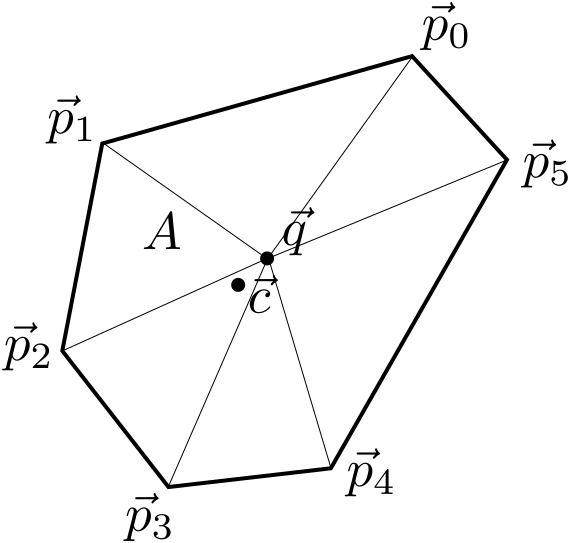
\includegraphics[width=0.35\textwidth]{pics/polygon.pdf}
  \caption{Polygon main properties computations}
  \label{fig:polygon}
\end{figure}

Now we can calculate the centers of mass of each triangle as
\begin{equation}
  \pnt{c}_i = ( \pnt{p}_i + \pnt{p}_{(i+1)'} + \pnt{q} ) / 3, \qquad
  (i+1)' = (i+1)\bmod N.
\end{equation}
And areas $A_i$ of each triangle and total area $A$.
\begin{equation}
  A_i = |(\pnt{p}_i - \pnt{q})\times (\pnt{p}_{(i+1)'} -
  \pnt{q})|,\qquad
  A = \sum_{i=0}^{N-1} A_i.
\end{equation}
Now, the center of mass can be computed as a sum of area-weighted
center of masses for each triangles:
\begin{equation}
  \pnt{c} = \sum_{i=0}^{N-1} A_i\pnt{c}_i / A.
\end{equation}
Total geometric moment of inertia (it is a moment of inertia divided
by mass) around center of mass is computed by same weighted approach:
\begin{equation}
  I/m = \sum_{i=0}^{N-1} A_i \left( (\pnt{p}_i-\pnt{c})^2 + 
  (\pnt{p}_{(i+1)'}-\pnt{c})\cdot (\pnt{p}_i-\pnt{c}) +
  (\pnt{p}_{(i+1)'}-\pnt{c})^2\right ) / (6A).
\end{equation}

\section{Mass}

Total mass need to be calculated up to at each timestep using the ice
thickness distribution function $g(h)$. General formula is
\begin{equation}
  m = \sum_{k=0}^{K-1} g(h_k) h_k\rho_k A,
\end{equation}
where $\rho_k$ is the density of ice of thickness $h_k$.

%=====================================================================
%%% File: wind.tex

\chapter{Wind Interpolation}

%----------------------------------------------------------------------

\section{Introduction}

The wind data is given in a mesh and, possibly, in some set of random
points. We have to be able to restore the proper wind vector for any
ice element on a sphere. We also would like to have a few analytical
testing fields that we can use. This chapter describes all that
related to the wind.

%----------------------------------------------------------------------

\section{Analytitcal Testing Fields}

First field to use is taken from~\cite{bib:fuselier2009stability},
field~1, pp.~3233--3234.

%=====================================================================
\newcommand{\Div} {\nabla\cdot}
\newcommand{\Vecsymb}[1] {{\boldsymbol{#1}}}
\newcommand{\ddt}[1] {{\partial #1 \over \partial t }}
\newcommand{\Grad} {\nabla}


%FILE: coordinates.tex

\chapter{Force Balance on Ice Elements}

During the Arctic Ice Dynamics Joint Experiment (AIDJEX) it was found that long term mean ice motion, in the summer when ice concentration is low, results from the balance of four forces on the ice \cite{Hunkins75, McPhee79}. In free drift the significant forces on the ice  are wind stress,   ocean stress, the Coriolis force and acceleration down the sea surface tilt. Inertial terms were found to be an order of magnitude smaller than these on daily or longer time scales \cite{Thorndike86}, however are important on shorter time scales and accumulative impact of the inertial motion of the ocean and ice maybe significant in the sea ice mass balance \cite{HeilandHibler2002}. The residual term in the measured force balance is found to be comparable to the Coriolis force, and an order of magnitude smaller than the wind stress \cite{McPhee79}. This residual is attributed to interactions between ice floes. In areas of ice convergence, resistance to compression becomes important, and ice can no longer be considered to be in free drift. For climatological studies small time scale forcing may be ignored. Contributions to the force balance from tidal motion, pressure gradients and inertial terms are considered to be small when averaged over time scales greater than a day \cite{McPhee79}. For short term ice drift estimation, and in regions with strong tides the tidal and inertial terms may become important. 

The force balance on the ice, per unit area, is given by: 
{\color{red} *** This needs to be replaced with force balance on an ice element. It needs to be integrated over the element area for surface forces and volume for body forces. We need to replace $\Div{\Vecsymb{\sigma}}$ with contact forces.***.}
% 
\begin{equation} 
\label{Ueqn}
    \ddt{m \Vec{U}} + \Div{ \left ( m \Vec{U} \Vec{U} \right )} = 
     \Vecsymb{\tau}_a + \Vecsymb{\tau}_w - m f \hat{\Vec{k}} \times \Vec{U} - m g \Grad H
    + \Div{\Vecsymb{\sigma}} ,
\end{equation}
%
where $m$ is the ice mass, $\Vec{U}$ is the ice velocity, $\Vecsymb{\tau}_a$ and $\Vecsymb{\tau}_w$ are the wind stress and ocean stress on the ice, $f$ is the Coriolis parameter, $\Vec{\hat{k}}$ is a unit vector normal to the surface, $g$ is the acceleration due to gravity and $H$ is the sea surface dynamic height. The remaining term $\Div{\Vecsymb{\sigma}}$ is a force due to sub-scale interactions between ice floes. A constitutive law defining the ice stress $\Vecsymb{\sigma}$ will be outlined in section \ref{rheologysection}. By scale analysis \cite{Hibler79} it can be shown that the advection of momentum, $\Div{(m\Vec{U}\Vec{U})}$ is two orders of magnitude smaller than the coriolis and gravitational terms and may be  neglected. The inertial term $\ddt{m\Vec{U}}$ is also small on time scales greater than a day. The momentum may be found from the balance between external forces and $\Div{\Vecsymb{\sigma}}$, which is the form \cite{Tremblay&Mysak1997} take for their model. The two largest terms, $\Vecsymb{\tau}_a$ and $\Vecsymb{\tau}_w$, are of the order $1 \, \mathrm{kg m^{-1} s^{-2}}$, and tend to oppose each other. The Coriolis, gravitational and interaction terms are of the same order of magnitude, and typically an order of magnitude smaller than $\Vecsymb{\tau}_a$ and $\Vecsymb{\tau}_w$. 

{\color{red}*** Need to re-write the above to reflect the shorter timescale we will resolve with Siku. And to write in terms of contact mechanics rather than continuum form. We also need to discuss inertial motion. The ice/ocean does manifest inertial oscillations in response to storms, it is the motion of the massive ocean that is causing the ice to oscillate. Which is not possible to model with out a coupled ice/ocean model. ***}

\section{Surface Forcing}

The force balance on an ice element includes stresses to the upper (atmosphere) and lower (ocean) surfaces that must be prescribed. 

The stress applied over a unit area of ice by the wind and ocean current is modelled with a quadratic boundary layer model \cite{Brown79,McPhee_Smith,McPheeJPO}. Ice velocity is an order of magnitude smaller than the wind velocity and insignificant when calculating the wind stress over the ice,
%
\begin{equation}
    \Vecsymb{\tau}_a = \rho_a C_a |\Vec{U}_a| 
          \left ( \Vec{U}_a \mathrm{cos} \theta_a + 
          \hat{\Vec{k}} \times \Vec{U}_a \mathrm{sin} \theta_a \right ) ,
\end{equation}
%
\begin{equation}
    \Vecsymb{\tau}_w = \rho_w C_w |\Vec{U}_w - \Vec{U}| 
         \left ( \left (\Vec{U}_w - \Vec{U} \right ) \mathrm{cos} \theta_w +
         \left (\Vec{U}_w - \Vec{U} \right ) \hat{\Vec{k}} \times \mathrm{sin} \theta_w
         \right ) .
\end{equation}
%
The drag laws require the air velocity, $\Vec{U}_a$, at a known height in the atmosphere and the ocean current, $\Vec{U}_w$, usually below the surface Ekman layer, to be known. It is possible to take these as geostrophic velocities, though they could equally well be provided at heights within the boundary layer by atmospheric and oceanic models. The other variables are the density of air, $\rho_a$; density of water, $\rho_w$; the drag coefficients for the air and water interfaces, $C_a$ and $C_w$; and the turning angles across the boundary layers, $\theta_a$ and $\theta_w$. The magnitude of the drag parameters and turning angle is dependent upon the height (depth) that winds (currents) are provided for.

{\color{red} *** Let's start with the simplist implimentation for drag coefficients and turning angles, assuming they are constant. $C_a$ and $C_w$ could be modeled as a function of ice morphology following \cite{Tsamadosetal2014}, and they can be adjusted to better fit observed ice drift following \cite{Kreysher??}. I also need to consider a version of the atmospheric stress parameterisation that allows for an unstable atmosphere boundary layer. This will take me a couple of days to sort out in my head. So beware, we may be replacing the wind stress equation with something else.}

For testing it is appropriate to start with the default values for the parameterisations. These are $C_w = 0.0045$, $\theta_w = 0$, $C_a=0.0016$ and $\theta_a= 0$. We are assuming the velocities are sufficiently close to the surface that Eckmann turning is negligable.

%
\section{Data Input}
% 

Wind and ocean current data can be sourced from various agencies. Either forecast model output can be used or reanalysis fields. Provided data is provided on a known grid SLERP (see section ??) will interpolate the fields to ice element locations.

%
\subsection{Winds}
%

Siku is set up to run with $10\,\mathrm{m}$ winds by default. It is possible to use geostropic winds or winds from different atmospheric levels, however to do this the drag parameterisation and turning angles will have to be adjusted in Siku's calculation of surface stress. {\color{red} *** ANTON: I assume we will have a lookup table variables are read in from where these can be set ***.}

Example wind fields are provided with the Siku distribution for testing purposes. 

%
\subsection{Ocean Currents}
%

{\color{red} *** Will provide information as soon as we have narrowed down which fields we shall use from Hycom or RASM. We should also include a note about adding tides to the currents, which could be provided by \cite{Kowalik&Proshutinsky??} for example. ***}

For testing purposes one can set the ocean currents to zero. In this can the ice is moving over a stationary ocean that provides drag. 

%=====================================================================
%%% File: diagnostics.tex

\chapter{Diagnostics}

Diagnostics is a facility to calculate and output some values from the
model on a set of coordinates.

For each diagnostics, the user registers a function in python script
where the data from diagnostics will be transferred to. Together with
this function, the user provides and registers set of points,
a.k.a. ``mesh'' where the data will be calculated. The user also
schedules the runs such that diagnostics will be performed only when
necessary, not at each time step.

%=====================================================================
%%% File: freedrift.tex

\chapter{Drift testing}

%----------------------------------------------------------------------

\section{Introduction}

It is obvious that our program should contain basic tests with easily 
observable results. These tests can either confirm that all calculations
are correct or show up that there are some miscalculations or phisical
laws which are not taken into account.

For proper testing we provide several simple tests, which could be ran
directly from 'freedrift.py', and some more complicated hardcoded tests, 
which require rebuilding the C++ core, that should not be made by users. 
More detailed description will be given below.

%----------------------------------------------------------------------

\section{User-restricted tests}

\subsection{Hardcoded winds}

In order to remove any possibilities to make a mistake while passing 
wind data from file to python and from python to core - a simple windfield 
has been hardcoded into C++ modules.

That field gives wind velocity by default equal to (-10, 1) in convention 
(east-velo, north-velo) in current velocity units all around the globe.
The values of components can be changed in module 'vecfield.cc' in method
'get\_at\_lat\_lon\_rad. This test can be turned on in module 'globals.hh':
one should uncomment testing constructor (next to atmospheric wind data 
declaration), and by default is turned off.

As the result - all elements on the globe should behave according to 
hardcoded wind. \textbf{NOTICE: hardcoded wind will not be outlined as
it is not connected with python!}

\subsection{Hardcoded spins}

In early stages, while interaction between elements is not properly 
defined, the most basic spin test has been hardcoded. The test is naive 
constant angular velocity of all elements. This velocity is brutally 
embedded inside 'dynamics.cc' module. The values are chosen for different
elements` behavior (and equal to zero by default). 

When angular velocity is small - elements behave like 'leaves on the wind',
simply drifting in direction of wind velocity, but slower in the reason 
of water. 
In the case of medium angular velocity - elements begin to turn aside from
wind direction while they are mowing. This effect is caused by some 
kind of inner model gyro forces.
When angular velocity is too high - elements behave more like spinning top:
they are moving slowly with fluctuations or not moving at all.
\textbf{NOTICE: angular velocity and as the result elements behavior 
depends on time scaling of current computing session!}

%----------------------------------------------------------------------

\section{Generic python tests}

\subsection{Output settings}

Befor starting the test itself, one should set a proper output for results.
In order to observe the results we provide besic GMT picturing called from 
python modules.

All preruntime picture settings are located in 'plot\_config.py' file and 
are optional.Most values have several samples and described below:
\begin{itemize}
\item 'uwind\_file' and 'vwind\_file' - string that contains the name of 
 .nc files with uwind and vwind variables. 'gmt\_plotter.py' automaticly
 prints wind grid from that files.
\item time\_index - integer, that specifies the time from .nc files for
 selecting the wind grid.
 \textbf{Totally optional: runtime setting provided}
\item 'grid\_step\_lat' and 'grid\_step\_lon' - grid steps in .nc files for 
 proper interpoaltion and plotting.
\item 'out\_pic\_name' - name of file for GMT output.
 \textbf{Totally optional: runtime setting provided}
\item 'verbose' - verbosity state
\item 'inter\_domain' - the domain for gmt\_plotter inner interpolation.
 Is being given in convention (minlon, maxlon, minlat, maxlat) in degrees.
 Several main domains are provided and commented out.
\item 'inter\_density' - average density of additional interpolated vectors
 in degrees. 0 - for canceling additional interpolation.
\item 'view' - \textbf{Important!} main option! Contains information about
 map projection, oriantation and other minor gmt settings.
 Various views are provided and commented out.
\item 'ground\_colr' - color of ground.
\item 'coasts' - \textbf{Important!} second main option, but generally
 optional as it has good dafault value.
 Contains gmt command string for printing coast lines.
\item 'vector\_scaling' - additional scaling for wind vectors.
 For most maps dafeult value suits well, but when entire globe is being 
 printed - vectors can cover all other output, so should be resized 
 manually.
\item 'inter\_wind' - gmt command line for printing interpolated winds. File
 name is synchronized with interpolation module.
\item 'grid\_wind' - gmt command line for printing grid winds. File
 name is synchronized with interpolation module.
\item 'underlays' and 'overlays' - lists of optional underlays and overlays
 (accordingly), such as monitoring output, additional grids or objects.
\end{itemize}

\subsection{Testing scenarios}

Same to all other scenarios - these are being set inside user scenario 
python files that are given as an argument to core binary (siku) on 
execution.

Current testing scenario settings are being contained in 'freedrift.py', 
and are described below.

\subsection{Materials}

Each element has various properties. A lot of them can be simply described
the material, which element is made of. 

Default material for model is ice.  Material`s parameters can be changed in 
'material.py'. Inside the scenario file all materials are being loaded into 
table in 'Define material' section.

\subsection{Wind initializations}

Befor anything can move one should define a wind grid for inner processing.
Yet only NMC reanalysis data is supported. 

Grid loading ang preprocessing examples are being located in 
'Wind initializations' section of 'freedrift.py'.
First of all one should load siku.wind field as a proper NMCSurfaceVField
object, that depends on two NMCVar objects for two wind components 
(described in 'wnd,py' and 'nmc.py' accordingly).
After the loading one can additionaly make some changes in that wind grid 
(such as setting all values equal to test values by 'make\_test\_field' 
method. It also can be applied after each loading or updating wind grid).

The 'make\_test\_field' method simply sets all values of wind velocity equal 
to that, which are given as arguments (in terms (east-velo, north-velo)).
If arguments are empty - the winds all over the glob will be set as huge 
cyclones. That is very usefull for checking global drift and spin either 
with or without detection land collisions. 

\subsection{Date/time}

As the model describes the dynamics - another inevitable setting is time.

Several time examples are being located in 'date/time settings' section 
in 'freedrift.py'. Generally time should be set by exact values, but
as every NMC file contains it`s own set of times, one can easily choose 
some elements from that set.

There are several time variables, that should be set:
\begin{itemize}
 \item siku.time.start - starting time of modelling
 \item siku.time.finish - finish time (modelling shall end after reaching 
 that time)
 \item siku.time.last - the time of last calculation step
 \item siku.time.last\_update - the time of last wind update (used by 
 wind updating methods)
 \item siku.time.dts - outer cumputation time limit. Program shall exit 
 after it would have been working for that amount of time.
 \item siku.time.dt - \textbf{Important!} time step of the model. This 
 value has huge influence on computing process (mostly by dynamics).
\end{itemize}

\subsection{Poligons}

All elements are being represented as geometric poligons with different 
properties. Most general methods (such as loading) are being provided by 
'Polygon' class. The object of that class is being initialized in 
'Polygon initialization' siction.

\subsection{Elements}

The most basic example of several simple elements is being located in 
'elements' section. 

Firstly one shoud set a list of vertices for each element.
Secondly one have to init each element as an object of 'Element' class
using 'Polygon' object, matching material and set of thicknesses specifying 
monitoring functions.
In the third place one should append these elements to the list of elements.

\subsection{Monitoring function}

The variables and methods in section 'Monitor function for the polygon'
are being used for monitoring (such as picturing) some (or all) of the 
elements. 

Currently there are next objects:
\begin{itemize}
 \item siku.plotter - an object of GMT\_Plotter class for picturing frames
 with GMT.
 \item diagnostics.monitor\_freq - testing variable, defines frequency
 (actually period) of making frames in units of timestem, thus it is integer.
 \item siki.drift\_monitor - monitor function for elements.
 \item siku.diagnostics.step\_count - counter of diagnostics steps.
\end{itemize}

\subsection{Diagnostics}

The vatiables and methods for diagnostics are being located in 'Diagnostics 
function for the winds' section.

\textbf{Currently not used}

\subsection{Callback}

All python methods are being called from C++ core as a call-back functions.
Therefore this methods has been declared in 'Callback flag-mask generator'
section and defined afterward.

These functions are:
\begin{itemize}
 \item siku.callback.pretimestep - functions, that is called befor main 
 camputations. Contains different preprocessings, such as wind updating.
 
 Currently updating is turned off because time step is too large and couse 
 unwanted updates spoiling results.
 \item siku.callback.aftertimestep - function, that is called after main
 computations. 
 
 Currently contains picturing of elements and winds.
 \item conclusions - function, that is called only once - befor program 
 exits. 
 
 Currently contains command for creating a .gif animation from all frames.
\end{itemize}

\subsection{Current testings}

Current version of freedrift.py contains scenario for testing global 
movement and spinning. Running the model with that scenario should make
255 time steps covering 55 days, create 51 .eps file with the locations of 
three poligons and finally make .gif animationt of their movement. 

Expected work time is about 30-60 seconds (mostly spent for picturing).

For drift testing with real winds one should comment out last 3 lines in 
'Wind initializations' section in 'freedrift.py'. That will set testing 
wind grid with povided .nc files.

For changing projection one should comment out current 'view' variable 
in 'plot\_config.py' and uncomment that view, which one wants to see 
(or define his own).

%----------------------------------------------------------------------

%=====================================================================
%%% File: mesh.tex

\chapter{Random points generation}


%----------------------------------------------------------------------

\section{Problem Statement}

We need to generate a set of points on sphere that will serve the role
of nuclei for Voronoi tesselation procedure. The set needs to satisfy
the following conditions:
\begin{enumerate}
\item
  The point set need to be randomly generated with some distribution
  (resolution) function over sphere. This means that some areas will
  have finer resolution than others.
\item
  The point set need to have blue noise characteristics. This means
  that the minimum distance between two points cannot exceed some
  limit value $d_{\min}$. This limit value is also a function of
  location.
\item
  The boundaries need to be also correctly represented. This means
  that the set of points need to contain explicitly the points from
  the boundaries. The resolution near the boundaries should be set by
  resolution function.
\end{enumerate}

The problem is not trivial. The standard approaches for generation of
blue noise are not always applicable here. On the other hand, we do
not need too sophisticated approach as the statistical quality of the
final set is not that critical.

The points are generated with \texttt{mesh/gen\_points.py} script that
is maintained to satisfy the procedure described in this chapter.

%----------------------------------------------------------------------

\section{Random points on sphere}


\subsection{Uniform distribution on sphere}\label{sec:marsaglia}

To generate a uniform point distribution a trivial random number
generation in the cube $(x,y,z)$ does not work. To pick a random point
on sphere we use the method by~\cite{bib:marsaglia1972}. The random
point $(x,y,z)$ on a sphere is generated using the following rule:
\begin{enumerate}
\item Generate X and Y, uniformly distributed on a segment (-1,1).
\item Reject all the points that $X^2+Y^2\ge 1$.
\item Generate a point on a sphere from the remaining points as
  follows:
\begin{equation}
  \begin{aligned}
    x &=& 2X\sqrt{1 - X^2 - Y^2},\\
    y &=& 2Y\sqrt{1 - X^2 - Y^2},\\
    z &=& 1 - 2(X^2+Y^2)
  \end{aligned}
\end{equation}
\end{enumerate}

\subsection{Blue noise}\label{sec:bluenoise}

The blue noise point generation is when the points are almost randomly
generated but with additional condition that there is no two points
that are closer than a particular distance $d_{\min}$. The simplest
way to generate blue noise is to remove a subset of the points from
the original set such that a new set will satisfy the blue noise
condtion. We proposed the following algorithm for this.

\begin{enumerate}
\item
  Sort all the points by $x$ coordinates (we will compare the
  projection of the points on $x$-axis).
\item
  Form a new empty list that will contain the blue noise set. Add the
  first point from the original list to it.
\item
  Traverse the original list starting from its second point. For each
  original point check the points from the new list backwards until
  the projection distance is smaller than $d_{\min}$. If no points are
  actually closer than $d_{\min}$, add original point to the new
  list. Otherwise, skip it.
\end{enumerate}

The new list will obviously satisfy the blue noise condition.

\subsection{Large voids}

There is no garantee that some points will be too isolated from the
set with much voids around. This problem can be solved by adding
points in the voids. However, we will not address it for now.

\subsection{Changing the distribution}

However, we need to generate the point set with varying distribution
function.

The first and simplest approach would be to generate the point set
with the finest resolution possible. Then we can apply the blue noise
filter technique described in Sec.~\ref{sec:bluenoise}. However, this
can be extremely slow even for not so fine resolution.

Instead, we can set the areas with different resolutions and the
simplest way is to generate uniform resolution in that areas and then
apply filter to the whole globe.

\subsection{Uniform distribution is selected region}

The method from Sec.~\ref{sec:marsaglia} cannot be directly
apply. However, we can use different approach. Technically, the
uniform distribution over the globe can be generated by
%
\begin{equation}
  \theta = 2\pi u, \quad \phi=\arccos( 2v-1 ),
\end{equation}
%
where $u$ and $v$ are random values on $(0,1)$.

%=====================================================================

\appendix
%=====================================================================
%FILE: formulas.tex

\chapter{Formulas Summary}

\paragraph{Dynamics}

\begin{equation}\label{eq:dynamicsH-x}
  \dot{\vct{\Omega}} = \vct{H} = \left( -\frac{F_y}{mR}, \frac{F_x}{mR},
  \frac{N}{I} \right)^T.
\end{equation}
\begin{equation}
  \vct{\Omega}^{n+1/2} = \vct{\Omega}^{n-1/2} + \Delta t\,\vct{H}^n.
\end{equation}

\paragraph{Placement}

\begin{equation}\label{eq:positionomega-x}
  \untqtrn{\dot q} = \frac{1}{2}\untqtrn{q}\circ\vct{\Omega},
\end{equation}
\begin{equation}
  \untqtrn{p} = \left(1 - \frac{\Omega^2\,\Delta t}{16} + \frac{\Delta
    t}{2}\,\vct{\Omega} \right) / \left( 1 +\frac{ \Omega^2\,\Delta
    t^2}{16}\right),
\end{equation}
\begin{equation}
  \untqtrn{q}^{n+1} = \untqtrn{q}^{n} \circ \untqtrn{p}.
\end{equation}


%=====================================================================
% FILE: quats.tex

\chapter{Quaternions and Rotations}\label{ch:qandrot}

%----------------------------------------------------------------------
\section{Briefly about Quaternions}

\cite{bib:graf2008quaternions} gives a good introduction to
quaternions and their application to represent rigid body
rotations. Here we will represent a few facts that will be useful in
future discussions. Most of the proofs will be omitted.

\subsection{Definitions}

A quaternion is a number system that extends the complex
numbers. Quaternions are 4-dimensional linear vector space over real
numbers with scalar product and quaternion product defined on
it. Algebraic definition similar to complex numbers is the
following. A quaternion $\bm{q}$ is defined as
\begin{equation}
  \bm{q} = q_0 + q_1 i + q_2 j + q_3 k,\qquad q_l \in \mathbb{R},\quad
  l=0,1,2,3,
\end{equation}
where $i^2=-1$ (same as with complex numbers), $j^2=k^2=ijk=-1$. The
multiplication of quaternion is non-commutative. That is the main
distinction of them with complex numbers.

$q_0$ is said to be a real value and $q_1$, $q_2$, and $q_3$ to be
imaginary values. The quaternion product ${}\circ{}$ of two
quaternions can be algebraically derived from these rules.

\subsection{Vector representation}

Quaternions can be represented in different form as a pair of a number
and a vector as follows
\begin{equation}
  \bm{q} = ( q_0, \vec{q} ), \qquad \Re{\bm{q}} = q_0, \qquad
  \Im{\bm{q}}=\vec{q}.
\end{equation}
The quaternion product of two quaternions $\bm{q}$ and $\bm{p}$ can be
defined in this notation as follows
\begin{equation}\label{eq:quatproduct}
  \bm{q}\circ\bm{p} = (q_0p_0-\vec{q}\cdot\vec{p},
  q_0\vec{p} + p_0\vec{q} + \vec{q}\times\vec{p}).
\end{equation}

\subsection{Vectors as quaternions}

Vectors can be considered to be quaternions with 0 real part. For two
vectors $\vec{a}$ and $\vec{b}$ we have
\begin{equation}
  \vec{a}\circ\vec{b} = ( -\vec{a}\cdot\vec{b}, \vec{a}\times\vec{b} ).
\end{equation}
Thus, quaternion product contains both dot- and cross-products of
vectors.

\subsection{Norm}

Norm of the quaternion is defined as follows
\begin{equation}
  |\bm{q}| = \left( q_0^2 + \vec{q}\cdot\vec{q} \right)^{1/2} = 
  \left( q_0^2 + q_1^2 + q_2^2 + q_3^2 \right)^{1/2}.
\end{equation}
It can be shown that
\begin{equation}
  |\bm{q}\circ\bm{p}| = |\bm{q}||\bm{p}|.
\end{equation}

\subsection{Conjugate}

The conjugate $\bm{\bar{q}}$ of quaternion $\bm{q}$ is defined as
\begin{equation}
  \bm{\bar{q}} = (q_0, -\vec{q}).
\end{equation}
It can be shown that
\begin{equation}
\bm{\bar{q}}\circ\bm{q} = \bm{q}\circ\bm{\bar{q}} = |q|^2.
\end{equation}

\subsection{Unit quaternions}

Thus, unit quaternions such that $|q|=1$ form a subalgebra of
quaternions over quaternion product operation. It can be shown that
the quaternion is unit if and only if it can be represented in the
following form
\begin{equation}
  \bm{q} = \left( \cos\frac{\psi}{2}, \sin\frac{\psi}{2}\,\vec{e}
  \right), \qquad |\vec{e}|=1.
\end{equation}
$\psi$ is known as ``rotation angle'' and unit vector $\vec{e}$ is
known as ``rotation axis vector''.

\subsection{Coordinate transformations using quaternions}

Let $\vec{a}$ be a vector represented in the Global frame
$\{x,y,z\}$. Let $\vec{A}$ be the same vector represented in local
coordinate system $\{X,Y,Z\}$. In this case it can be shown that
coordinate transformations between two systems can be expressed as
follows:
\begin{equation}\label{eq:transform}
  \vec{A} = \bar{\bm{q}}\circ \vec{a} \circ \bm{q},\qquad
  \vec{a} = \bm{q}\circ \vec{A} \circ \bar{\bm{q}}
\end{equation}

%----------------------------------------------------------------------
\section{Rotation Matrix and Positions}\label{sec:rotquat}

An important problem (mostly for visualization) is to determine
spherical coordinates $(\phi,\lambda)$ of an element polygon vertex by
quaternion $\bm{q}$ of the polygon and vertex local coordinates
$(X_i,Y_i)$. When local coordinates of the vertex $\vec{P}=(X,Y,Z)^T$
are known, the global coordinates can be found as follows:
\begin{equation}
  \vec{p} = \bm{R}\cdot\vec{P},
\end{equation}
where $\bm{R}$ is 3D rotational matrix restored from quaternion.
The formulas can be found in many places, for example in a general
introduction \cite{bib:wikipedia-quaternions-srotation}. For rotation
matrix $R$ and quaternion $\hat q$ with elements $(s,v_x,v_y,v_z)$ we
have
\begin{equation}
  R({\hat q}) = 
    \begin{pmatrix}
      q_0^2 + q_1^2 - q_2^2 - q_3^2 & 2q_1 q_2 - 2 q_0 q_3 & 2q_1 q_3 + 2 q_0 q_2\\
      2q_1 q_2 + 2 q_0 q_3 &  q_0^2 - q_1^2 + q_2^2 - q_3^2 & 2q_2q_3-2q_0q_1 \\
      2q_1 q_3 - 2 q_0 q_2 &  2q_2q_3+2q_0q_1 & q_0^2 - q_1^2 - q_2^2 + q_3^2 \\
    \end{pmatrix},
\end{equation}
or in a more computationally convenient way
\begin{equation}
  R({\hat q}) = 
    \begin{pmatrix}
      1 - 2q_2^2 - 2q_3^2 & 2q_1 q_2 - 2 q_0 q_3 & 2q_1 q_3 + 2 q_0 q_2\\
      2q_1 q_2 + 2 q_0 q_3 &  1 - 2q_1^2 - 2q_3^2 & 2q_2q_3-2q_0q_1 \\
      2q_1 q_3 - 2 q_0 q_2 &  2q_2q_3+2q_0q_1 & 1  - 2q_1^2 - 2q_2^2 \\
    \end{pmatrix}
\end{equation}
The most efficient way to perfom these computations was found
in~\cite{bib:geometrictools-rotation-performance}. We just use
standard libraries available for these transformation.

%=====================================================================

%=====================================================================
\bibliographystyle{apalike} 
\bibliography{siku}\label{sec:bibliography}

\end{document}
